\documentclass[pdftex,12pt,a4paper]{report}

\usepackage[pdftex]{graphicx}
\usepackage{enumitem}
\usepackage{fmtcount}
\usepackage{multirow}
\usepackage[margin=0.8in]{geometry}
\usepackage{verbatim}
\usepackage{moreverb}
\usepackage{listings}
\usepackage{color}
\usepackage{xcolor}
\usepackage{textcomp}
\usepackage{caption}
\usepackage{array}


\definecolor{listinggray}{gray}{0.9}
\definecolor{lbcolor}{rgb}{0.9,0.9,0.9}
\lstset{
	backgroundcolor=\color{lbcolor},
	tabsize=4,
	rulecolor=,
	language=C++,
        basicstyle=\scriptsize,
        upquote=true,
        aboveskip={1.5\baselineskip},
        columns=fixed,
        showstringspaces=false,
        extendedchars=true,
        breaklines=true,
        prebreak = \raisebox{0ex}[0ex][0ex]{\ensuremath{\hookleftarrow}},
        frame=single,
        showtabs=false,
        showspaces=false,
        showstringspaces=false,
        identifierstyle=\ttfamily,
        keywordstyle=\color[rgb]{0,0,1},
        commentstyle=\color[rgb]{0.133,0.545,0.133},
        stringstyle=\color[rgb]{0.627,0.126,0.941},
}


\renewcommand{\thefootnote}{\arabic{footnote}}
\newcommand{\HRule}{\rule{\linewidth}{0.5mm}}

\begin{document}


\begin{titlepage}
\begin{center}

\begin{minipage}{0.4\textwidth}
\begin{flushleft}

\includegraphics[width=0.6\textwidth]{./logo_telecom.jpg}
\end{flushleft}
\end{minipage}
\begin{minipage}{0.4\textwidth}
\begin{flushright} \large

\includegraphics[width=0.7\textwidth]{./arm.jpg}\\
ARM Ltd. \\                                                                
110 Fulbourn Road \\
Cambridge \\
GB-CB1 9NJ \\
Great Britain \\
\end{flushright}
\end{minipage}\\[1.5cm]

% Upper part of the page

\includegraphics[width=0.3\textwidth]{./mbed.jpg}\\[1.5cm]

\LARGE Industrial Placement Report\\[0.5cm]
% Title
\HRule \\
{ \huge \bfseries Embedded systems: \\ From a local connectivity to the cloud}\\

\HRule \\[1cm]

% Author and supervisor
\begin{minipage}{0.4\textwidth}
\begin{flushleft} \large
\emph{T\'{e}l\'{e}com Paristech mentor:}\\
Samuel \textsc{Tardieu}
\end{flushleft}
\end{minipage}
\begin{minipage}{0.4\textwidth}
\begin{flushright} \large
\emph{Supervisor:} \\
Simon \textsc{Ford}
\end{flushright}
\end{minipage}\\[1.0cm]


\begin{minipage}{0.4\textwidth}
\begin{center} \large
\emph{Author:} \\
Samuel \textsc{Mokrani}
\end{center}
\end{minipage}\\[3.0cm]

\large This report summarises the work I did during my T\'{e}l\'{e}com ParisTech engineering internship. I worked at ARM, more precisely in the Mbed team, from the 4th of July 2011 until the 3rd of February 2012.



\vfill

% Bottom of the page
{\large \today}

\end{center}

\end{titlepage}
\tableofcontents
\chapter{ARM and Mbed}
\section{ARM}
ARM Holdings plc is a British multinational semiconductor and software company. The headquarter is based in Cambridge. This company is well-known in the processor field, although it also designs, licenses and sells software development tools under the RealView and KEIL brands, systems and platforms, system-on-a-chip infrastructure and software. 
\\

Advanced RISC Machines Ltd (now ARM Ltd) was founded in November 1990. It is the result of a joint venture between Acorn Computers, Apple Computer (now Apple Inc.) and VLSI Technology (now NXP semiconductor). The purpose of this joint venture was to develop a RISC chip originally developped by Acorn Computer involved in an Apple project. ARM got bigger little by little by acquiring companies like Micrologic Solutions, a software consulting company based in Cambridge 1999. In 2000, ARM acquired Allant Software, Infinite Designs in Sheffield (UK) and EuroMips in Sophia Antipolis (France). Then, in 2001, it acquired a team specialized in hardware and software debugging based in Blackburn (UK). In 2005, ARM acquired Keil Software, a leader in the software development tools for microcontrollers. More recently, ARM joined with Texas Instrument, Samsung, IBM, ST-Ericsson and Freescale Semiconductor in forming an open source engineering company named Linaro. Linaro produces for example ARM tools or linux kernels for ARM based system-on-chips. Today, ARM has offices and design centres all over the world, including UK, Germany, France, Israel, Sweden, Norway, Slovenia, USA, China, South Korea, Japan, Taiwan and India. 
\\

Nowadays, ARM processors are widely used in mobile phones, tablets, personal digital assistants, GPS, digital cameras and digital televions. The main reason of this success is their low electric power consumption; making them suitable for embedded systems. Even if ARM products are widely used, the company doesn't manufacture its own CPUs. The company licenses its technology as Intellectual Property (IP). Companies like Intel, Texas Intrument or Nvidia are making processors based on ARM's IP.



\section{Mbed}
In wish to pursue new areas of expertise, ARM founded Mbed in 2009. Mbeds core area is development of prototyping boards (called mbed) based on ARM processors (Cortex M0 and Cortex M3). The purpose is to make available a simple and easy to set-up prototyping solution using 32-bits processors. Mbeds boards have been designed for quick experimentation. Users can try something and see if it is doable in a very easily and quickly manner.

\subsection{Mbed boards}
For the moment, three boards have been developped. The first one is based on the LPC2368 microcontroller from NXP which uses a Cortex m3. The second is based on a LPC1768 (Cortex m3). More recently, a new board based on a LPC11U24 (Cortex m0) was born. This last mbed has been particularly designed to prototype USB devices or battery powered applications. 

\begin{figure}[h!]
\centering
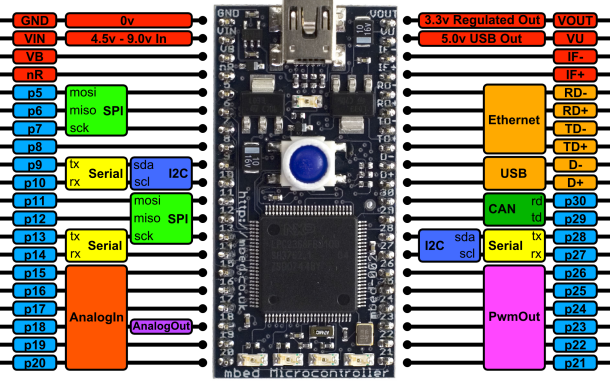
\includegraphics[width=0.5\textwidth]{./lpc1768.png}
\caption{mbed board: lpc1768 (cortex m3)}
\label{mbed_board: lpc1768 (Cortex m3)}
\end{figure}

\begin{figure}[h!]
\centering
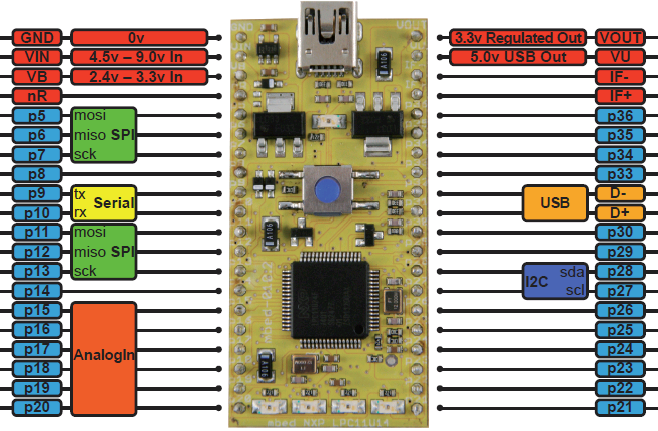
\includegraphics[width=0.5\textwidth]{./lpc11U24.png}
\caption{mbed board: lpc11U24 (cortex m0)}
\label{mbed_board: lpc11U24 (Cortex m0)}
\end{figure}


\subsection{The online compiler}
The two main keywords of Mbed are "simple" and "cloud computing". Users indeed use an online compiler to develop their program in C++. They compile online and transfer the binary received into the mbed, which is connected to a computer over a USB cable and detected as a mass storage device. They just have to press the reset button to see their program running.
\\

As explained before, users have a complete online IDE totally independant of the underlying operating system. 
This IDE has a lot of very interesting features:
\begin{itemize} \itemsep 0em
	\item Code editing with syntax highlighting
	\item Multiple programs
	\item Import programs from online catalogue of published programs
	\item Import programs from zip file
	\item Full output of compile-time messages
	\item Multiple target support
	\item Publish your code directly from the compiler
	\item Export your programs as a .zip file
	\item Build information including graphical display of code size and RAM usage
	\item Code formatter
	\item Import and update of libraries from SVN
	\item Version control: you can commit, revert, update, merge your programs
\end{itemize}

\subsection{Mbed libraries}
In addition to the online compiler, almost all drivers have been implemented. Users just have to instanciate an object such as SPI, I2C,... to have access to a great API which abstract all the low-level layer. \\


\begin{figure}[h!]
\centering
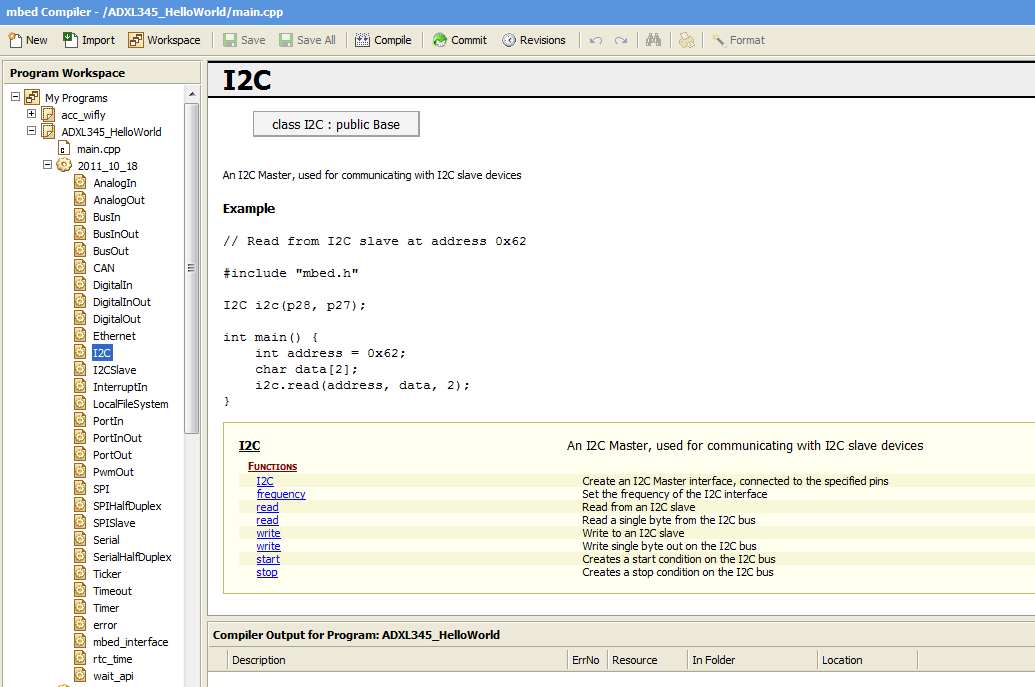
\includegraphics[width=0.7\textwidth]{./libraries.png}
\caption{mbed libraries}
\label{mbed libraries}
\end{figure}


\subsection{Mbed website: \textit{http://mbed.org/}}
To finish this tour of the mbed environment, users can find an active website. First, users have access to a forum. They have also access to a handbook where there is a lot of documentation and examples concerning mbed libraries, the hardware part of the mbed,... But the most important feature of this website is for me the central cookbook. This cookbook is a great source of example coming from other mbed users. You can almost find for instance a lot of libraries to use popular sensors like accelerometers, pressure sensors,... Each user is free to contribute to this part of the website by doing articles explaining their project. 

\begin{figure}[h!]
\centering
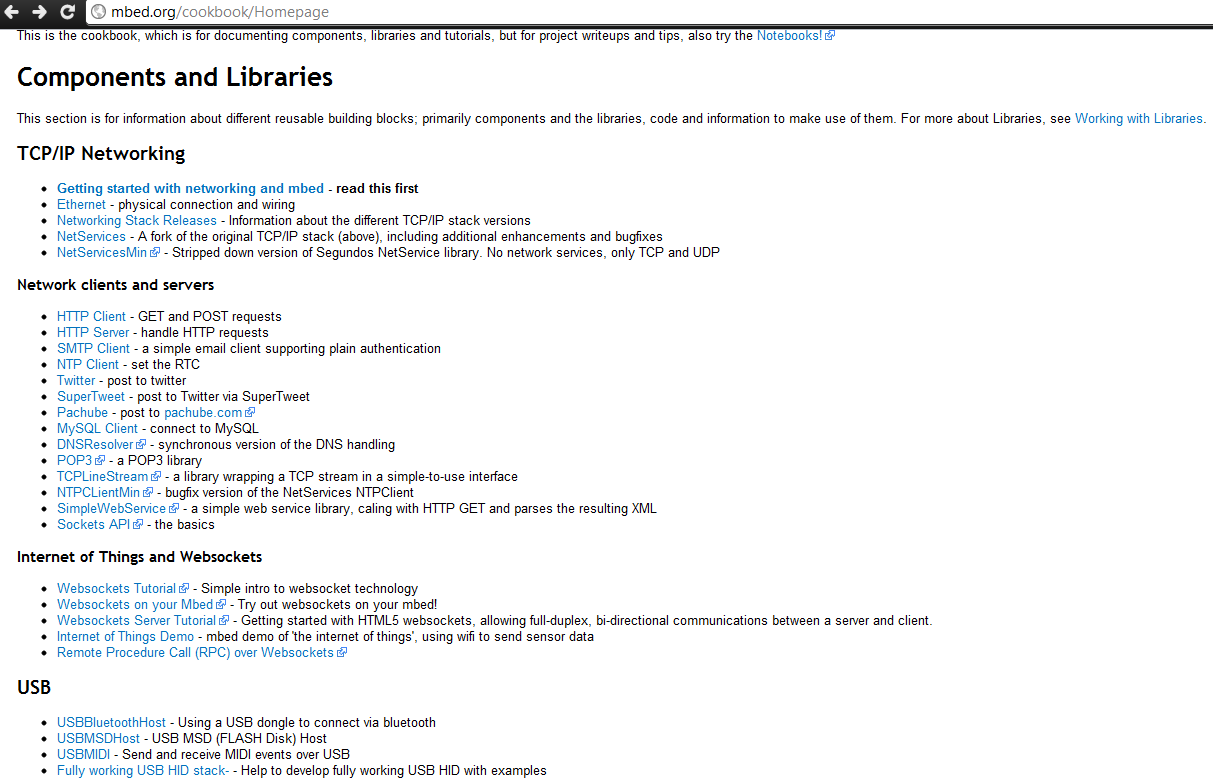
\includegraphics[width=0.7\textwidth]{./cookbook.png}
\caption{mbed cookbook}
\label{mbed cookbook}
\end{figure}


\chapter{Internet Of Things: internet device boom}
Nowadays, an increasing number of devices are connected to the Internet. These devices include not only personal computers, but also mobile phones and digital televisions, ect.
Cisco predicts in an interview from the BBC that the number of internet connected devices is set to explode in the next four years to over 15 billion - twice the world's population by 2015. And Cisco is not the only one company to predict a such boom. VMware's CEO Paul Maritz said during a speech at the annual VMworld conference in Las Vegas in August 2011 that:

\begin{quote} "Three years ago over 95 percent of the devices connected to the Internet were personal computers. Three years from now that number will probably be less than 20 percent. More than 80 percent of the devices connected to the Internet will not be Windows-based personal computers." \\
\end{quote}

Thus, working on the connection of different sensors to the Internet is becoming more and more crucial. I will describe in this chapter two projects concerning the Internet of Things: real-time data streaming from sensors and Remote Procedure Call mechanism. Both of these projects use a new feature of HTML5: a Webscoket communication.

\section{Websockets}
\subsection{Introduction}
The WebSocket specification is a new feature of HTML5. It defines a full-duplex single socket connection over which messages can be sent between client and server. The WebSocket standard simplifies much of the complexity around bi-directional web communication and connection management. Furthermore, it reduces polling and unnecessary network throughput overhead. 

\begin{figure}[h!]
		\centering
		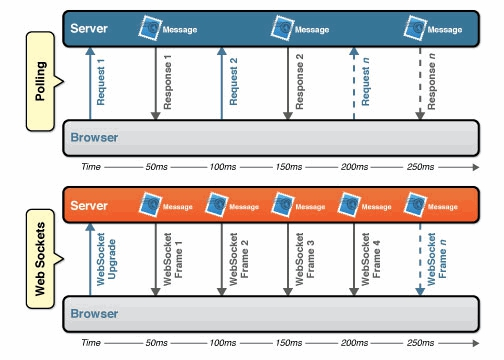
\includegraphics[width=0.7\textwidth]{./ws_poll.jpg}
		\caption{Reduction of polling and overhead by Websocket \textit(Image coutesy of Kaazing)}
		\label{Reduction of polling and overhead by Websocket}
\end{figure}

This figure shows the reduction in latency. Once the connection is established, messages can flow from the server to the browser. As the connection remains open, there is no need to send another request to the server.

\subsection{Websocket protocol}

To establish a WebSocket connection, the client and server upgrade from the HTTP protocol to the WebSocket protocol during their initial handshake. There are several handshake mechanisms. Here I present the basic handshake of one of them; the websocket protocol 76, which has been  implemented in mbed websocket library:


The handshake from the client looks as follows: \\

\fbox{\begin{minipage}{1.0\textwidth} \small
	GET /ws HTTP/1.1 \\
	Host: example.org \\
  Connection: Upgrade \\
  Sec-WebSocket-Key2: 12998 5 Y3 1  .P00 \\
  Upgrade: WebSocket \\
  Sec-WebSocket-Key1: 4 @1  46546xW\%0l 1 5 \\
  Origin: http://example.org \\ \\
  \^{}n:ds[4U
  \end{minipage}
}
\\ \\
The handshake from the server looks as follows: \\

\fbox{\begin{minipage}{1.0\textwidth} \small
        HTTP/1.1 101 WebSocket Protocol Handshake \\
        Upgrade: WebSocket \\
        Connection: Upgrade \\
        Sec-WebSocket-Origin: http://example.org \\
        Sec-WebSocket-Location: ws://example.org/ws \\ \\
        8jKS'y:G*Co,Wxa-
        \end{minipage} 
        }
\\ \\
Once the Websocket connection is established, data can be exchanged according to this format:
\begin{itemize} \itemsep 0em
	\item Send a 0x00 byte
	\item Encode the message using UTF-8 and send the resulting byte stream
	\item Send a 0xFF byte
\end{itemize}

\subsection{Architecture of a Websocket communication}
A websocket communication involves several clients connected to the same websocket server. All messages from browsers are sent to the server. The server manages all messages. It can decide to send a message received from a client to another client, to broadcast all messages received to all clients connected,...


\begin{figure}[h!]
		\centering
		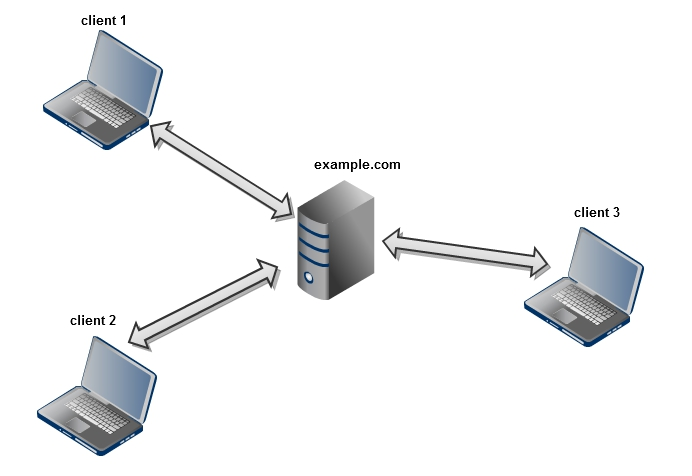
\includegraphics[width=0.7\textwidth]{./ws.jpg}
		\caption{Example of websocket communication}
		\label{Example of websocket communication}
\end{figure}

For instance, let's say that there is an existing websocket server: example.com which is listening on port 80. A client can open a connection, receive and send messages to this server with this few lines of javascript:

\begin{center}
\begin{lstlisting}[label=Device descriptor,caption=Device Descriptor]
var ws = new WebSocket("ws://example.com");
ws.onopen = function(evt) { 
   alert("Connection open"); 
   ws.send("Hello")}; 
};
ws.onmessage = function(evt) { 
   alert( "Message received: " + evt.data); 
}; 
ws.onclose = function(evt) { 
   alert("Connection closed."); 
};
\end{lstlisting}
\end{center}


\section{Real-Time Streaming Data from sensors}
\section{Remote procedure Call over Websockets}
	
	
	
	
	
	
	
	
	
	
	
	
	
	
	
	
	
	
	
	
	
	
	

\chapter{Universal Serial Bus}
\section{USB overview}
The Universal Serial Bus (USB) is the most widely used bus in today's computer. USB has particularly been designed to standardize connections between the computer and peripherals. For instance, keyboards, printers, scanners, disk drives or cameras can use the same bus to exchange data with a computer. USB has effectively replaced a variety of earlier interfaces, such as serial or parallel ports. The most useful advantage is certainly the plug-and-play nature it has. In other words, you can connect and disconnect devices on your computer without the need to restart it.\\

USB version 1.0 supported two speeds, a full speed mode of 12Mbits/s and a low speed mode of 1.5Mbits/s. USB 2.0, which is the most widely version of USB, can reach 480Mbits/s. The 480Mbits/s is known as High Speed mode. USB version 3.0 specifies a maximum transmission speed of up to 5Gbits/s (known as SuperSpeed), but few products are supporting USB 3.0 at present.
\\
\begin{table}[h!]
\begin{center}
\begin{tabular}{|l|l|l|}
\hline
\multirow{2}{*}{USB 1.0} & low-speed & 1.5Mbits/s \\
 & full-speed & 12Mbits/s \\ \hline
USB 2.0 & high-speed & 480Mbits/s \\ \hline
USB 3.0 & super-speed & 5Gbits/s \\ \hline
\end{tabular}
\end{center}
\caption{USB speeds}
\label{USB speeds}
\end{table}

The Universal Serial Bus is host controlled. However, there can only be one host per bus and the host is responsible for undertaking all transactions. Considering this restriction, two devices cannot exchange information without one host. Nevertheless, the On-The-Go specification, which is part of the USB 2.0 standard, has introduced a Host Negotiation Protocol, allowing two devices to negotiate for the role of host. With this specification, we can imagine a camera exchanging data with a printer without the need of a computer. 

\section{How does the USB work?}
\subsection{Topology}
The physical bus topology defines how USB devices are connected to the host. The USB network is implemented as a tiered star network with one host (master) and several devices (slaves). The topology looks like a tree. In order to increase the number of devices connected, a hub need to be connected to the root port. This special hub and the root port are the first tier of the network. Furthermore, the USB network can support up to 127 external nodes but the number of tiers does not exceed 7. The following diagram represents a possible connection architecture on a USB bus.


\begin{figure}[h!]
		\centering
		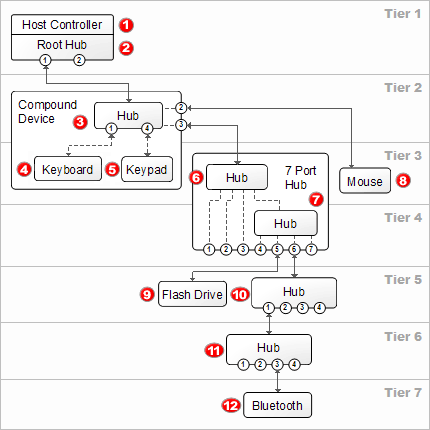
\includegraphics[width=0.5\textwidth]{./usb_topology.png}
		\caption{USB physical topology \footnotemark}
		\label{USB physical topology}
\end{figure}
\footnotetext{reference: http://www.usblyzer.com}
\subsection{Endpoints}
Devices have a series of buffers to communicate with the host. Each buffer will belong to an endpoint. An endpoint is a uniquely identifiable entity on a USB device, which is the source or terminus of the data that flows from or to the device. For instance, the mbed based on a NXP LPC1768 microcontroller has 32 physical endpoints whereas the mbed based on the NXP LPC11U24, has 10 physical endpoints. One physical endpoint represents two logical endpoints. Each physical endpoints has a specific direction: either OUT to receive data from the host or IN to send data to the host. 
\\
There are four types of endpoints: 
\begin{itemize}
	\item \textbf{Control endpoint}: All USB devices once connected performed an \textit{enumeration step} wherein the host request all capabilities of the device. Control transfers are used to enumerate a device.
	\item \textbf{Interrupt endpoints}: Interrupts transfers are used when a device requires responsiveness. Typical applications would include keyboard and mouse. Users don't want a noticeable delay between pressing a key or moving a mouse and seeing the result on the screen. An interrupt transfer only occurs when the host polls the device. There is a guarantee that the host will request a data within a specified time interval
	\item \textbf{Bulk endpoints}: Bulk transfers are typically used to transfer large amount of data like files to a printer. A bulk transfer use spare un-allocated bandwidth, so time is not critical with bulk transfers. Typical applications include printers and scanners.
	\item \textbf{Isochronous endpoints}: Isochronous tranfers are used for streaming and real time data. For instance, USB speakers uses isochronous tranfers. Such devices need a guaranteed delivery rate for data but errors can occur.
\end{itemize}
	
\begin{figure}[h!]
		\centering
		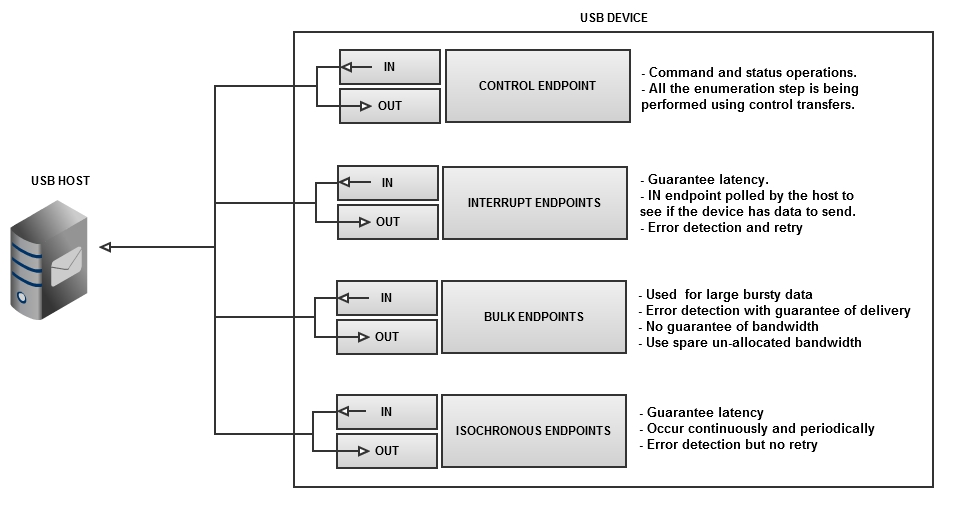
\includegraphics[width=1.0\textwidth]{./endpoint.jpg}
		\caption{Different types of endpoints}
		\label{Different types of endpoints}
\end{figure}

\subsection{Packets exchanged}
\subsubsection{\underline{Common fields in a USB packet}}

\begin{table}[h!]
\centering
\begin{tabular}{|c|c| >{\centering\arraybackslash}m{9cm} |}
\hline
Field & Length & Meaning \\ \hline
\multirow{2}{*}{SYNC} & low and full speed: 8bits  & \multirow{2}{10cm}{A packet starts with a SYNC pattern to allow the receiver bit clock to synchronise with the data.} \\
\cline{2-2}%
 & high speed: 32bits & \\ \hline
 
EOP &  & A packet ends with an End of Packet (EOP) field \\ \hline

PID & 8bits & Packet ID \\ \hline

\multirow{2}{*}{ADDR} & \multirow{2}{*}{7bits} & The address field specifies which device the packet is designated for\\ \hline

\multirow{2}{*}{ENDP} & \multirow{2}{*}{8bits} & The endpoint number which the packet is designed for \\ \hline

\multirow{2}{*}{CRC} & \multirow{2}{*}{5 or 16bits} & Cyclic Redundancy Checks are performed on the data within the packet payload \\ \hline
\end{tabular}
\caption{Fields in a USB packet}
\label{Fields in a USB packet}
\end{table}

\subsubsection{\underline{Packets}}
\begin{itemize}
	\item \textbf{Token Packet}: To indicate the type of transaction to follow, USB uses token packets:
		\begin{center}
		\begin{tabular}{|c|c|c|c|c|c|}
  	\hline
  		SYNC & PID & ADDR & ENDP & CRC5 & EOP \\ \hline
  		8/32bits & 8bits & 7bits & 4bits & 5bits &  \\
  	\hline
  	\end{tabular}
  	\end{center}
  	
  	There are three types of token packets: 
  	\begin{itemize} \itemsep 0em
			\item IN: The host wants to read information.
			\item OUT: The host wants to send information.
			\item SETUP: Used to begin control transfers.
  	\end{itemize}
  	
  	
	\item \textbf{Data Packet}: Packets which contain the payload
		\begin{center}
		\begin{tabular}{|c|c|c|c|c|}
  	\hline
  		SYNC & PID & DATA & CRC16 & EOP \\ \hline
  		8/32bits & 8bits & (0 - 1024) * 8bits & 16bits &   \\
  	\hline
  	\end{tabular}
  	\end{center}
  	
  	
	\item \textbf{Handshake Packet}: After a data stage, handshake packets are used to acknowledge data or to report errors
		\begin{center}
		\begin{tabular}{|c|c|c|}
  	\hline
  		SYNC & PID & EOP \\ \hline
  		8/32bits & 8bits &  \\
  	\hline
  	\end{tabular}
  	\end{center}
  	
  	There are four types of handshake packets:
  	\begin{itemize} \itemsep 0em
			\item ACK: Packet successfully received.
			\item NAK: The device temporary cannot send or received data
			\item STALL: Endpoint is halted, or control pipe request is not supported.
			\item NYET: No response yet from receiver (high speed only)
  	\end{itemize}
  	
  	
	\item \textbf{Start of Frame Packet}: USB manages time in units called "frames" (USB 2.0 further added "microframes"), and uses frames/microframes to realize the concept of time. Each "frame" represents 1 ms, and each microframe represents 125 microseconds. When performing control, bulk or interrupt transfers with a peripheral device, there is little need to pay attention to the frames/microframes. However, when performing isochronous transfers, frames/microframes may need to be taken into consideration for proper synchronization with the system. For this reason, the host issues SOF (Start Of Frame) packets to the bus to indicate the starting point of each frame/microframe.
	
		\begin{center}
		\begin{tabular}{|c|c|c|c|c|}
  	\hline
  		SYNC & PID & Frame number & CRC5 & EOP \\ \hline
  		8/32bits & 8bits & 11bits & 5bits &   \\
  	\hline
  	\end{tabular}
  	\end{center}
  	
  	
\end{itemize}

\subsection{USB data flow}

\begin{figure}[h!]
		\centering
		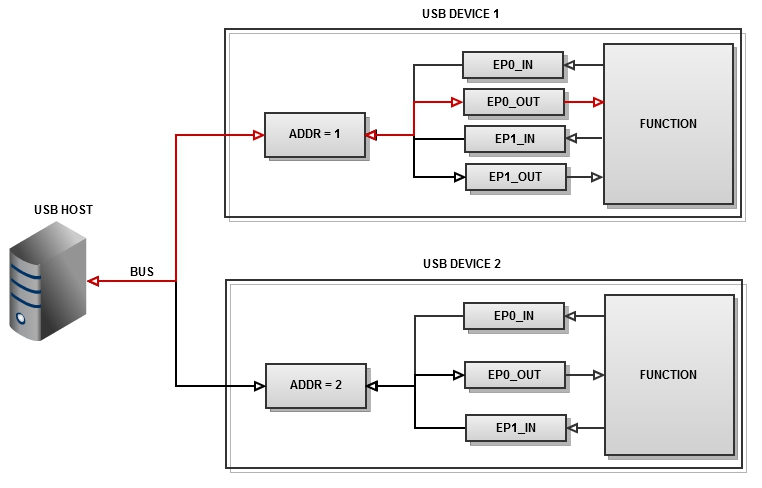
\includegraphics[width=1.0\textwidth]{./data_flow.jpg}
		\caption{From the host to a device}
		\label{From the host to a device}
\end{figure}

Say for example, the host sends a packet to device=2, endpoint=1OUT. The function hardware will read the request and determine from the address field whether the packet is for itself, and if so will copy the payload of the following data packet to the appropriate endpoint buffer. It will then send a handshake packet to acknowledge the reception of the byte and generate an internal interrupt within the microcontroller for the appropriate endpoint signifying it has received a packet. This is typically all done in hardware.
\\

\subsection{Enumeration}
The host hub port is able to detect the attachment of the USB device and makes the host controller aware of the same. The host controller then starts communicating with the USB device (which could be a mouse, keyboard, flash drive etc.). This initial communication between the host and the device is termed as �bus enumeration�. Bus enumeration is the process through which the host learns about the capabilities of the device. Since any USB device can be connected to the host hub port at anytime, bus enumeration becomes the essential first step of USB communication. This step is performed on the control endpoint (endpoint 0). So, all devices must at least have a control endpoint (endpoint 0) enabled.
During this step, the host will assign a unique address to the device.
All devices capabilities are transmitted in data structures called \textit{descriptors}. Descriptors are arrays containing some information like the device class, the number of endpoints used, the maximum length of these endpoints,... There are several types of descriptors. Standards descriptors are: device descriptor, configuration descriptor, interface descriptor and endpoint descriptor. But, for each USB class, other descriptors can be found such as the HID (Human Interface Device)descriptor and the report descriptor for HID devices.
\\

\begin{figure}[h!]
		\centering
		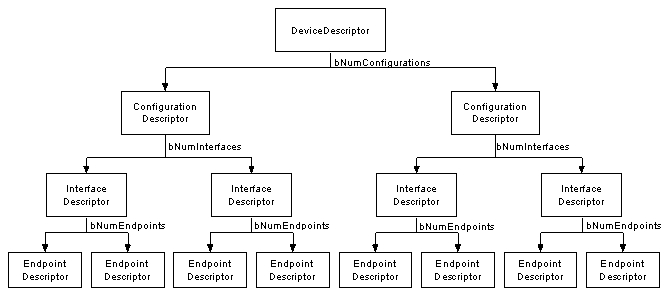
\includegraphics[width=0.7\textwidth]{./descr.jpg}
		\caption{Descriptors}
		\label{Descriptors}
\end{figure}

A typical enumeration follows:
\begin{itemize}
	\item GET DEVICE DESCRIPTOR: The host sends a get device descriptor request. The device
replies with its device descriptor to report its attributes (Device Class, maximum packet size for endpoint zero).
	\item SET ADDRESS: A USB device uses the default address (0) after reset until the host assigns a unique address using the set address request. The firmware writes the device address assigned by the host.
	\item GET CONFIGURATION DESCRIPTOR: The host sends a get configuration request. The device replies with its configuration descriptor, interface descriptor and endpoint descriptor. The configuration descriptor describes the number of interfaces provided by the configuration, the power source
(Bus or Self powered) and the maximum power consumption of the USB device from the bus.
The Interface descriptor describes the number of endpoints used by this interface. The Endpoint
descriptor describes the transfer type supported and the bandwidth requirements.
	\item SET CONFIGURATION: The host assigns a configuration value to the device based on the
configuration information. The device is now configured and ready to be
used.
\end{itemize}


\newpage
\section{USB Device stack}
A USB device stack has been developped to allow mbed users to design their own USB device or to use their mbed as USB peripheral such as a keyboard or a mouse. USB defines class code information that is used to identify a device�s functionality. This class code is parsed by the USB host stack to load an appropriate device driver. Two widely used USB classes has been implemented: HID (Human Interface Device) and MSD (Mass Storage Device). Users have access to a subset of a third class known as CDC (Communication Device Class). This class is particularly used to design a virtual serial port over USB. The following diagram shows the software architecture of this stack.

\begin{figure}[h!]
		\centering
		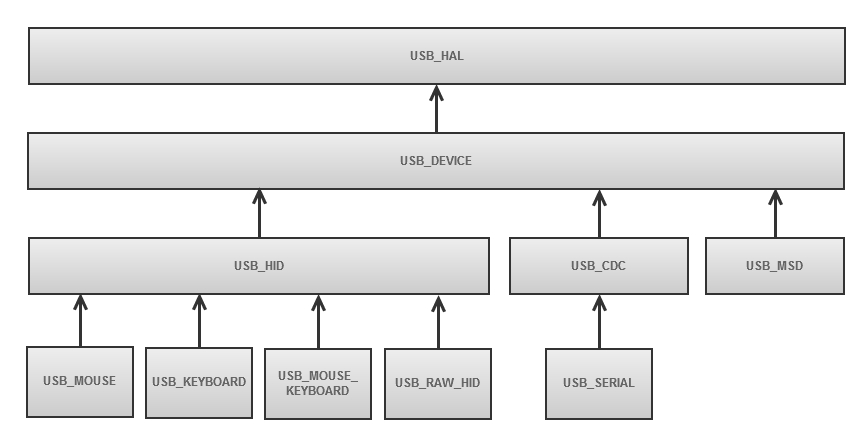
\includegraphics[width=1.0\textwidth]{./usb_stack.jpg}
		\caption{USB device stack architecture}
		\label{USB device stack architecture}
\end{figure}

As in all stacks, it is organized by layers:
\begin{itemize}
	\item USBHAL: The USB hardware layer. All low levels methods are on this class. We found in particular the USB interrupt handler and methods to initialize the USB controller, read or write a certain endpoint. This class defines also virtual methods which are executed each time that there is an interrupt concerning a packet received or the end of a writing so that a child class can use them to perform their own treatment when a such event occurs.
	\item USBDEVICE: This layer is in charge to abstract the hardware. Methods such as init, connect, disconnect, addEndpoint, readEndpoint, writeEndpoint can be found in this class. It's also in this class that the enumeration step is performed for requests concerning standard descriptors. When a packet is received on the control endpoint (endpoint 0 OUT), it is decoded to analyze the request and a response to the host is sent. Descriptors are accessible via virtual functions such as getDeviceDescriptor which returns a pointer on the descriptor. As these functions are virtual, all child classes will be able to use their own descriptors.
		\item USBHID, USBCDC and USBMSD: As explained before, these classes represent a specific USB class. A part of the enumeration step can be done here if the host requests a class specific descriptor. These three classes are explained in the next section of this document.
		\item USB\_MOUSE, USB\_KEYBOARD, USB\_MOUSE\_KEYBOARD, USB\_RAW\_HID and \\ USB\_SERIAL: High level libraries to emulate a specific peripheral according to their class. For instance, a keyboard is emulated over the HID class. Methods such as printf, putc are accessible for a keyboard. The USB\_RAW\_HID class is used to send and receive raw data. This can be a good opportunity to design a USB device. USB\_SERIAL is a virtual serial port.
\end{itemize}


\subsection{USBHAL}

\begin{center}
\textbf{Source code of main methods are in Annexe A: USBHAL class}
\end{center}


This section describes the hardware layer implemented for the mbed LPC11U24. This microcontroller has a built-in USB 2.0 device controller. It also has 2kbytes of RAM dedicated for USB operations. An important other feature the double buffering support for generic endpoints.

\begin{figure}[h!]
		\centering
		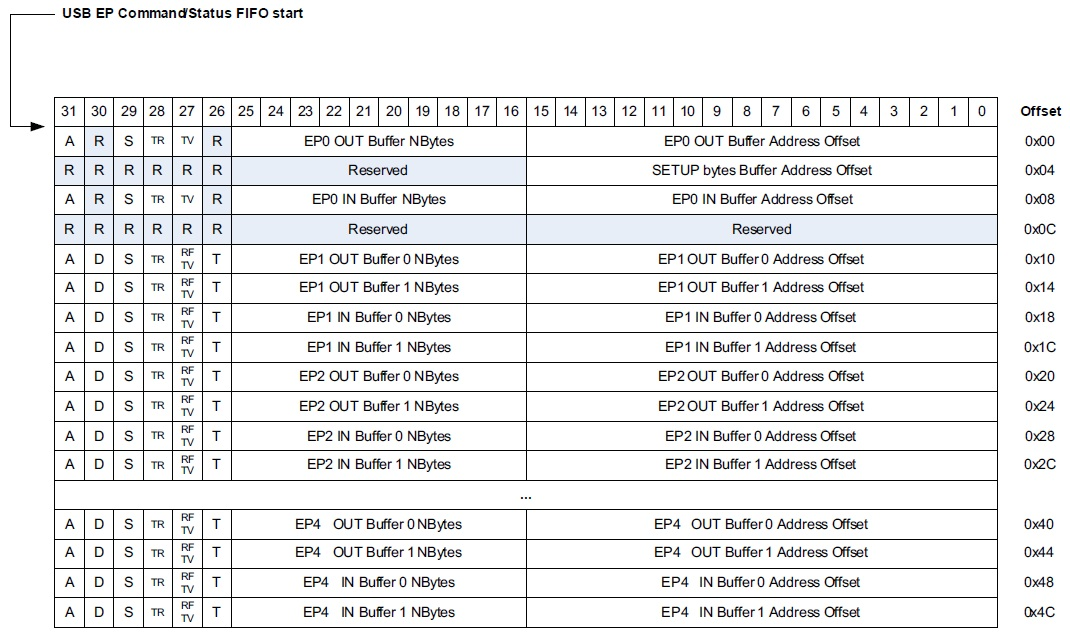
\includegraphics[width=1.0\textwidth]{./usb_endpoints.jpg}
		\caption{USB endpoints status array}
		\label{USB endpoints status array}
\end{figure}

To describe the state of each endpoints available, we need to allocate space in USB RAM as specified in the previous figure. Main fields of endpoints status array are:
\begin{itemize}
	\item A: the endpoint is active or not
	\item NBytes: For OUT endpoints this is the number of bytes that can be received in this buffer. For IN endpoints this is the number of bytes that must be transmitted.
	\item Address offset: represents the end of the address where will be stored data. The beginning of the address is specified in DATABUFSTART register 
\end{itemize}



Main methods for USBHAL class:
\begin{itemize}
	\item Memory  allocation for endpoints status list and endpoint 0 buffers. These initializations are done in the constructor of USBHAL::USBHAL.
	\item To add more endpoints, space allocation has to be done. This is done in the method: USBHAL::realiseEndpoint
	\item To read a specific endpoint:
		\begin{itemize}
			\item Fill the endpoint status list (active bit, address offset and NBytes). After this step, the endpoint is ready to receive data. This is done in USBHAL::endpointRead
			\item When a data is received on the specific endpoint, an interrupt is raised. Software can read data in the buffer of this OUT endpoint. This is done in USBHAL::endpointReadResult.
		\end{itemize}
	\item To write on a specific endpoint:
		\begin{itemize}
			\item Fill the endpoint status list (active bit, address offset and NBytes). Copy data in the buffer of the IN endpoint. After this step, the endpoint is ready to send data. This is done in USBHAL::endpointWrite
			\item Wait until the writing has been effectively done. This is done in USBHAL::endpoint-\\WriteResult.
		\end{itemize}
\end{itemize}


\section{HID class}
\subsection{Introduction}
HID is one of the most frequently used USB classes. The HID class was primarily defined for devices that are used by humans to control the operation of computer systems. Typical examples of HID class devices include keyboards, mice, trackballs, and joysticks. An HID device may have knobs, switches, buttons, sliders, etc. The HID class is also frequently used for devices that may not require human interaction but provide data in a similar format as HID class devices. Since all operating systems have a built-in HID driver, it's easy to design a USB HID device which doesn't require any specific driver.

Data exchanged between host and device resides in structure called reports. The report format is flexible and can handle any format of data, but each report has a fixed size. This size is specified in a HID descriptor which is transmitted as part of the configuration descriptor.
HID devices are required to provide a Report Descriptor which enumerates all data fields of a report. A HID device can have at most one interrupt IN endpoint and one interrupt OUT endpoint (and the control endpoint to perform the enumeration step).

For each field in the report, the Report Descriptor defines how many bits the field consumes, how often this data is repeated, and which is the type of the data field. Thus, report descriptors are specific to a device. Examples of report descriptor are provided in next sections of this document concerning HID devices such as mice or keyboards.
\\

Concerning standard descriptors, they are quite similar for all HID devices:
\begin{lstlisting}[label=Device Descriptor,caption=Device Descriptor]
uint8_t * USBDevice::deviceDesc() {
    static uint8_t deviceDescriptor[] = {
        DEVICE_DESCRIPTOR_LENGTH,       // bLength 
        DEVICE_DESCRIPTOR,              // bDescriptorType 
        LSB(USB_VERSION_2_0),           // bcdUSB (LSB) 
        MSB(USB_VERSION_2_0),           // bcdUSB (MSB) 
        0x00,                           // bDeviceClass 
        0x00,                           // bDeviceSubClass 
        0x00,                           // bDeviceprotocol 
        MAX_PACKET_SIZE_EP0,            // bMaxPacketSize0 
        LSB(VENDOR_ID),                 // idVendor (LSB) 
        MSB(VENDOR_ID),                 // idVendor (MSB) 
        LSB(PRODUCT_ID),                // idProduct (LSB) 
        MSB(PRODUCT_ID),                // idProduct (MSB) 
        LSB(PRODUCT_RELEASE),           // bcdDevice (LSB) 
        MSB(PRODUCT_RELEASE),           // bcdDevice (MSB) 
        STRING_OFFSET_IMANUFACTURER,    // iManufacturer 
        STRING_OFFSET_IPRODUCT,         // iProduct 
        STRING_OFFSET_ISERIAL,          // iSerialNumber 
        0x01                            // bNumConfigurations 
    };
    return deviceDescriptor;
}
\end{lstlisting}

\begin{lstlisting}[label=Configuration Descriptor,caption=Configuration Descriptor]
uint8_t * USBHID::configurationDesc() {
    static uint8_t configurationDescriptor[] = {
        CONFIGURATION_DESCRIPTOR_LENGTH,// bLength
        CONFIGURATION_DESCRIPTOR,       // bDescriptorType
        LSB(TOTAL_DESCRIPTOR_LENGTH),   // wTotalLength (LSB)
        MSB(TOTAL_DESCRIPTOR_LENGTH),   // wTotalLength (MSB)
        0x01,                           // bNumInterfaces
        DEFAULT_CONFIGURATION,          // bConfigurationValue
        0x00,                           // iConfiguration
        C_RESERVED | C_SELF_POWERED,    // bmAttributes
        C_POWER(0),                     // bMaxPower

        //Interface descriptor
        INTERFACE_DESCRIPTOR_LENGTH,    // bLength
        INTERFACE_DESCRIPTOR,           // bDescriptorType
        0x00,                           // bInterfaceNumber
        0x00,                           // bAlternateSetting
        0x02,                           // bNumEndpoints
        HID_CLASS,                      // bInterfaceClass
        HID_SUBCLASS_NONE,              // bInterfaceSubClass
        HID_PROTOCOL_NONE,              // bInterfaceProtocol
        0x00,                           // iInterface

        //hid descriptor
        HID_DESCRIPTOR_LENGTH,          // bLength
        HID_DESCRIPTOR,                 // bDescriptorType
        LSB(HID_VERSION_1_11),          // bcdHID (LSB)
        MSB(HID_VERSION_1_11),          // bcdHID (MSB)
        0x00,                           // bCountryCode
        0x01,                           // bNumDescriptors
        REPORT_DESCRIPTOR,              // bDescriptorType
        LSB(this->reportDescLength()),  // wDescriptorLength (LSB)
        MSB(this->reportDescLength()),  // wDescriptorLength (MSB)

        //endpoint descriptor (interrupt IN endpoint)
        ENDPOINT_DESCRIPTOR_LENGTH,     // bLength
        ENDPOINT_DESCRIPTOR,            // bDescriptorType
        PHY_TO_DESC(EPINT_IN),          // bEndpointAddress
        E_INTERRUPT,                    // bmAttributes
        LSB(MAX_PACKET_SIZE_EPINT),     // wMaxPacketSize (LSB)
        MSB(MAX_PACKET_SIZE_EPINT),     // wMaxPacketSize (MSB)
        10,                             // bInterval (milliseconds)

        //endpoint descriptor (interrupt OUT endpoint)
        ENDPOINT_DESCRIPTOR_LENGTH,     // bLength
        ENDPOINT_DESCRIPTOR,            // bDescriptorType
        PHY_TO_DESC(EPINT_OUT),         // bEndpointAddress
        E_INTERRUPT,                    // bmAttributes
        LSB(MAX_PACKET_SIZE_EPINT),     // wMaxPacketSize (LSB)
        MSB(MAX_PACKET_SIZE_EPINT),     // wMaxPacketSize (MSB)
        10,                             // bInterval (milliseconds)
    };
    return configurationDescriptor;
}
\end{lstlisting}

In the device descriptor, the host will find information such as the maximum packets length that can be exchanged over the control endpoint, the device identification (vendor\_id, product\_id and product\_release) and the USB version used.

In the configuration descriptor, we find particularly the interface descriptor which defines the class used by this device (HID\_CLASS) and the number of endpoints that will be used (2). The HID descriptor gives information on the length of the report descriptor. There are finally endpoint descriptors. The communication uses two interrupt endpoints: one IN to send data to the host and one OUT to receive data from the host. Interrupts endpoint are polled by the host, that is why there is a bInterval field in endpoint descriptors.
\\

Additionnally, this class defines methods to send and receive reports:

\begin{lstlisting}[label=Send and receive HID reports,caption=Send and receive HID reports]
bool USBHID::send(HID_REPORT *report)
{
    return USBDevice::write(EPINT_IN, report->data, report->length, MAX_HID_REPORT_SIZE);
}


bool USBHID::read(HID_REPORT *report)
{
    uint16_t bytesRead = 0;
    bool result;
    result = USBDevice::read(EPINT_OUT, report->data, &bytesRead, MAX_HID_REPORT_SIZE);
    if(!readStart(EPINT_OUT, MAX_HID_REPORT_SIZE))
        return false;
    report->length = bytesRead;
    return result;
}


bool USBHID::readNB(HID_REPORT *report)
{
    uint16_t bytesRead = 0;
    bool result;
    result = USBDevice::readNB(EPINT_OUT, report->data, &bytesRead, MAX_HID_REPORT_SIZE);
    report->length = bytesRead;
    if(!readStart(EPINT_OUT, MAX_HID_REPORT_SIZE))
        return false;
    return result;
}
\end{lstlisting}

\subsection{Generic HID device}
If a USBHID is instantiated, the device created is a generic HID device. This means that it is not a specific device such as a mouse or a keyboard but a device which can send and receive raw data. The report descriptor for this kind of device is:
 
\begin{lstlisting}[label=Generic HID Report Descriptor,caption=Generic HID Report Descriptor]
uint8_t * USBHID::reportDesc() {
    static uint8_t reportDescriptor[] = {
        0x06, LSB(0xFFAB), MSB(0xFFAB),
        0x0A, LSB(0x0200), MSB(0x0200),
        0xA1, 0x01,         // Collection 0x01
        
        //data are sent in packets containing input_length bytes
        0x75, 0x08,         // report size = 8 bits
        0x15, 0x00,         // logical minimum = 0
        0x26, 0xFF, 0x00,   // logical maximum = 255
        0x95, input_length, // report count
        0x09, 0x01,         // usage
        0x81, 0x02,         // Input (array)
        
        //data are received in packets containing output_length bytes
        0x95, output_length,// report count
        0x09, 0x02,         // usage
        0x91, 0x02,         // Output (array)
        
        0xC0                // end collection

    };
    return reportDescriptor;
}
\end{lstlisting}

There are two main parts:
\begin{itemize}
	\item Bytes are sent to the host by packets of length \textit{input\_length}
	\item Bytes are received by packets of length \textit{output\_length}
\end{itemize}

\subsection{USBMOUSE}
USBMOUSE class is a subclass of USBHID. The important descriptor of this class is the report descriptor which defines data structures which will be exchanged.


\begin{lstlisting}[label=Mouse Report Descriptor,caption=Mouse Report Descriptor]
uint8_t * USBMouse::reportDesc() {
    static uint8_t reportDescriptor[] = {
        USAGE_PAGE(1),      0x01,       // Generic Desktop
        USAGE(1),           0x02,       // Mouse
        COLLECTION(1),      0x01,       // Application
        USAGE(1),           0x01,       // Pointer
        COLLECTION(1),      0x00,       // Physical

        // Buttons
        REPORT_COUNT(1),    0x03,       // 3 buttons
        REPORT_SIZE(1),     0x01,       // 1 bit for each button
        USAGE_PAGE(1),      0x09,       // Buttons
        USAGE_MINIMUM(1),   0x1,    
        USAGE_MAXIMUM(1),   0x3,
        LOGICAL_MINIMUM(1), 0x00,       // Button not pressed
        LOGICAL_MAXIMUM(1), 0x01,       // Button pressed
        INPUT(1),           0x02,       // Input, absolute data
        REPORT_COUNT(1),    0x01,       // Padding to fill 1 byte (5 + 3)
        REPORT_SIZE(1),     0x05,
        INPUT(1),           0x01,
        
        // X, Y and scroll
        REPORT_COUNT(1),    0x03,       // 3 features: X, Y, scroll
        REPORT_SIZE(1),     0x08,       // 1 byte for X, 1 byte for Y and 1 byte for scroll
        USAGE_PAGE(1),      0x01,
        USAGE(1),           0x30,       // X
        USAGE(1),           0x31,       // Y
        USAGE(1),           0x38,       // scroll
        LOGICAL_MINIMUM(1), 0x81,       // Minimum: -127
        LOGICAL_MAXIMUM(1), 0x7f,       // Maximum: 127
        INPUT(1),           0x06,       // Input, Relative data

        END_COLLECTION(0),
        END_COLLECTION(0),
    };
    return reportDescriptor;
}
\end{lstlisting}

On this report descriptor, we can distinguish three different parts:
\begin{itemize}
	\item At the beginning, there is the indication that a mouse report descriptor will be described.
	\item Buttons mouse: There are 3 buttons represented by 1 bit. Values for these buttons are 0 or 1 (pressed or not). They are input values which means that the device will send information to the host.
	\item X, Y and scroll: 3 different features, each represented by 1 byte. Values can vary between -127 and 127. There are also input values.
\end{itemize}

The main method to send a mouse state to the host is:

\begin{lstlisting}[label=Mouse Report Descriptor,caption=Mouse Report Descriptor]
bool USBMouse::mouseSend(int8_t x, int8_t y, uint8_t buttons, int8_t z) {
    HID_REPORT report;
    report.data[0] = buttons & 0x07;
    report.data[1] = x;
    report.data[2] = y;
    report.data[3] = -z; // >0 to scroll down, <0 to scroll up

    report.length = 4;

    return USBHID::send(&report);
}
\end{lstlisting}


\section{CDC class}
\subsection{Introduction}
The Communication Device Class (CDC) is a general-purpose way to enable all
types of communications on the Universal Serial Bus (USB). This class makes it possible
to connect telecommunication devices such as digital telephones or analog
modems, as well as networking devices like ADSL or Cable modems.
While a CDC device enables the implementation of quite complex devices, it can also
be used as a very simple method for communication on the USB. For example, a CDC
device can appear as a virtual COM port, which greatly simplifies application programming
on the host side. For mbed a subset of the CDC class has been implemented in order to create
a virtual serial port over USB.

\subsection{Descriptors}
On this class, two interfaces are used:
\begin{itemize}
	\item \textbf{Communication Class Interface}: used to request and manage the device state. This interface is also used by the host to request capabilities and parameters of the communication. This interface requires the control endpoint for device management. Optionnally, an interrupt IN endpoint can be used yo send event notifications to the host3.
	\item \textbf{Data Class Interface}: this interface is used for data transfers. For the communication, either bulk or interrupt endpoints are required. For a serial port,  reliability
of the transmission is very important and the data transfers are not time-critical. That is why, two bulk endpoints (one IN and one OUT) are used.
\end{itemize}

\begin{lstlisting}[label=USBSerial device descriptor,caption=USBSerial device descriptor]
uint8_t * USBCDC::deviceDesc() {
    static uint8_t deviceDescriptor[] = {
        18,                   // bLength
        1,                    // bDescriptorType
        0x10, 0x01,           // bcdUSB
        2,                    // bDeviceClass (CDC)
        0,                    // bDeviceSubClass
        0,                    // bDeviceProtocol
        MAX_PACKET_SIZE_EP0,  // bMaxPacketSize0
        LSB(VENDOR_ID), MSB(VENDOR_ID),  // idVendor
        LSB(PRODUCT_ID), MSB(PRODUCT_ID),// idProduct
        0x00, 0x01,           // bcdDevice
        1,                    // iManufacturer
        2,                    // iProduct
        3,                    // iSerialNumber
        1                     // bNumConfigurations
    };
    return deviceDescriptor;
}
\end{lstlisting}
This device descriptor is very common. The only change is the bDeviceClass field which contains the CDC class code.

\begin{lstlisting}[label=USBSerial configuration descriptor,caption=USBSerial configuration descriptor]
uint8_t * USBCDC::configurationDesc() {
    static uint8_t configDescriptor[] = {
        9,                      // bLength;
        2,                      // bDescriptorType;
        LSB(CONFIG1_DESC_SIZE), // wTotalLength
        MSB(CONFIG1_DESC_SIZE),
        2,                      // bNumInterfaces
        1,                      // bConfigurationValue
        0,                      // iConfiguration
        0x80,                   // bmAttributes
        50,                     // bMaxPower


        // interface descriptor: Communication Class Interface
        9,                      // bLength
        4,                      // bDescriptorType
        0,                      // bInterfaceNumber
        0,                      // bAlternateSetting
        1,                      // bNumEndpoints
        0x02,                   // bInterfaceClass
        0x02,                   // bInterfaceSubClass
        0x01,                   // bInterfaceProtocol
        0,                      // iInterface

        // CDC Header Functional Descriptor, CDC Spec 5.2.3.1, Table 26
        5,                      // bFunctionLength
        0x24,                   // bDescriptorType
        0x00,                   // bDescriptorSubtype
        0x10, 0x01,             // bcdCDC

        // Call Management Functional Descriptor, CDC Spec 5.2.3.2, Table 27
        5,                      // bFunctionLength
        0x24,                   // bDescriptorType
        0x01,                   // bDescriptorSubtype
        0x03,                   // bmCapabilities
        1,                      // bDataInterface

        // Abstract Control Management Functional Descriptor, CDC Spec 5.2.3.3, Table 28
        4,                      // bFunctionLength
        0x24,                   // bDescriptorType
        0x02,                   // bDescriptorSubtype
        0x06,                   // bmCapabilities

        // Union Functional Descriptor, CDC Spec 5.2.3.8, Table 33
        5,                      // bFunctionLength
        0x24,                   // bDescriptorType
        0x06,                   // bDescriptorSubtype
        0,                      // bMasterInterface
        1,                      // bSlaveInterface0

        // endpoint descriptor
        ENDPOINT_DESCRIPTOR_LENGTH,     // bLength
        ENDPOINT_DESCRIPTOR,            // bDescriptorType
        PHY_TO_DESC(EPINT_IN),          // bEndpointAddress
        E_INTERRUPT,                    // bmAttributes (0x03=intr)
        LSB(MAX_PACKET_SIZE_EPINT),     // wMaxPacketSize (LSB)
        MSB(MAX_PACKET_SIZE_EPINT),     // wMaxPacketSize (MSB)
        16,                             // bInterval




        // interface descriptor: Data Class Interface
        9,          // bLength
        4,          // bDescriptorType
        1,          // bInterfaceNumber
        0,          // bAlternateSetting
        2,          // bNumEndpoints
        0x0A,       // bInterfaceClass
        0x00,       // bInterfaceSubClass
        0x00,       // bInterfaceProtocol
        0,          // iInterface

        // endpoint descriptor
        7,                      // bLength
        5,                      // bDescriptorType
        PHY_TO_DESC(EPBULK_IN), // bEndpointAddress
        0x02,                   // bmAttributes (0x02=bulk)
        LSB(MAX_PACKET_SIZE_EPBULK),    // wMaxPacketSize (LSB)
        MSB(MAX_PACKET_SIZE_EPBULK),    // wMaxPacketSize (MSB)
        0,                      // bInterval

        // endpoint descriptor
        7,                      // bLength
        5,                      // bDescriptorType
        PHY_TO_DESC(EPBULK_OUT),// bEndpointAddress
        0x02,                   // bmAttributes (0x02=bulk)
        LSB(MAX_PACKET_SIZE_EPBULK),    // wMaxPacketSize (LSB)
        MSB(MAX_PACKET_SIZE_EPBULK),     // wMaxPacketSize (MSB)
        0                       // bInterval
    };
    return configDescriptor;
}
\end{lstlisting}
Four CDC specific descriptors are used in this configuration descriptor:

\begin{itemize}
	\item CDCHeaderDescriptor: marks the beginning of the concatenated set of functional descriptors for the interface.
	\item CDCCallManagementDescriptor: describes the processing of calls for the Communication Class interface
 	\item CDCAbstractControlManagementDescriptor: describes the commands supported by the Communication Class interface. This device supports for instance the request GET\_LINE\_CODING which allows the host to know parameters of the communication (number of stop bits, parity, number of data bits)
	\item CDCUnionDescriptor: describes the relationship between a group of interfaces that can be considered to form
a functional unit. Here, the master interface is the Communication Class Interface and the slave one is the data Class Interface.
\end{itemize}

Otherwise, this descriptor contains the 2 interfaces, as expected. The first one uses one IN endpoint and the second one two bulk endpoints. 





\section{MSD class}
\subsection{Introduction}
The Mass Storage Device (MSD) class is an extension to the USB specification that defines
how mass storage devices, such as a hard-disk, SD card, flash chip should operate on the USB.
Many devices use the MSD class to symplify data transfer. More common devices which use this class are hard-drives, USB-stick, MP3 or video player.

\subsection{How the USB MSD class works ?}

\subsubsection{\underline{Endpoints used}}
This class uses three endpoints:
\begin{itemize}
	\item Control endpoint: used for the enumeration step and to unhalt others endpoints when an error occured. The MSD protocol indeed specifies that the device must halt endpoints which are used to transfer data when an error occurs. So the endpoint 0 is also used to return in a functionnal state.
	\item The other two endpoints are bulk endpoints as big amount of data is exchanged between host and device. They are used for transferring commands and data over the bus.
\end{itemize}

\subsubsection{\underline{MSD transaction}}
The communication between the device and the host is divided into three steps:
\begin{itemize}
	\item Command stage
	\item An optional data stage
	\item Status stage
\end{itemize}

The \textbf{command stage} is used by the host to transmit instructions to be performed by the device. These instructions are contained in a Command Block Wrapper (CBW) isent by the host. The CBW describes several parameters of the transaction:

\begin{table}[h!]
\centering
\begin{tabular}{|c|c|c| >{\arraybackslash}m{9cm} |}
\hline

Offset & Field & Length (bytes) & Meaning \\ \hline
0 & dCBWSignature & 4 & Signature to identify a valid CBW (0x43425355) \\ \hline
4 & dCBWTag & 4 &  id of the CBW. The device have to answer in the status stage by sending a Command Status Wrapper (CSW) containing the same id. \\ \hline
8 & dCBWTransferLength & 4 & Length of transfer \\ \hline
12 & bmCBWFlags & 1 & bit7: transfer direction (0: OUT, 1: IN) \\ \hline
13 & bCBWLUN & 1 & \textbf{Bits 0-3}: logical unit to which the command is sent \\ \hline
14 & bCBWCBLength & 1 & \textbf{Bits 0-5}: Length of command block in bytes \\ \hline
15 & CBWCB & 0-16 & Command block: instructions to be executed by the device \\ \hline

\end{tabular}
\caption{Command Block Wrapper (CBW)}
\label{Command Block Wrapper (CBW)}
\end{table}

When a CBW has been received and decoded by the device, an optional \textbf{data stage} may take
place if the command requires it. During this step, data flow from or to the device (for instance, if the host wants to read the content of an SD card, there will be a data IN stage). Several transfers can occur successively.
\\

Once the data stage performed, the device must send a Command Status Wrapper (CSW) in response to the CBW. A CSW is used to return the result of a command.

\begin{table}[h!]
\centering
\begin{tabular}{|c|c|c| >{\arraybackslash}m{9cm} |}
\hline

Offset & Field & Length (bytes) & Meaning \\ \hline
0 & dCSWSignature & 4 & Signature to identify a valid CSW (0x53425355) \\ \hline
4 & dCSWTag & 4 &  Same id as in the CBW \\ \hline
8 & dCSWDataResidue & 4 & Difference between expected and real transfer length \\ \hline
12 & bCSWStatus & 1 & Indicates the result (success or failure) of the command. \\ \hline

\end{tabular}
\caption{Command Status Wrapper (CSW)}
\label{Command Status Wrapper (CSW)}
\end{table}

\subsubsection{\underline{State machine}}
To implement the three previous step of a transaction, a state machine is used.
This state machine contains 5 states:
\begin{itemize}
	\item WAIT\_CBW: waiting for CBW reception
	\item PROCESS\_CBW: decode and execute command from the CBW
	\item SEND\_CSW: a CSW will be send
	\item WAIT\_CSW: waiting for CSW reception by the host
	\item ERROR: to report an error
\end{itemize}

TODO: put diagram of state machine

\subsection{Implementation of the USBMSD class}

\begin{center}
\textbf{Source code of main methods are in Annexe B: USBMSD class}
\end{center}
\subsubsection{\underline{Evolution of the state machine}}
Thanks to virtual functions called from USBHAL when an interrupt occurs, we are able to evolve our state machine. 

\begin{lstlisting}[label=State machine,caption=State machine]
// Called in ISR context when a data are received
bool USBMSD::EP2_OUT_callback() {
    uint16_t size = 0;
    uint8_t buf[MAX_PACKET_SIZE_EPBULK];
    read(EPBULK_OUT, buf, &size, MAX_PACKET_SIZE_EPBULK);
    switch (stage) {
        // the device has to decode the CBW received
        case READ_CBW:
            CBWDecode(buf, size);
            break;
        
        // the device has to receive data from the host
        case PROCESS_CBW:
            switch (cbw.CB[0]) {
                case WRITE10:
                case WRITE12:
                    memoryWrite(buf, size);
                    break;
                case VERIFY10:
                    memoryVerify(buf, size);
                    break;
            }
            break;
        
        // an error has occured: stall endpoint and send CSW
        default:
            stallEndpoint(EPBULK_OUT);
            csw.Status = CSW_ERROR;
            sendCSW();
            break;
    }

    //reactivate readings on the OUT bulk endpoint
    readStart(EPBULK_OUT, MAX_PACKET_SIZE_EPBULK);
    return true;
}

// Called in ISR context when data has been transferred
bool USBMSD::EP2_IN_callback() {
    switch (stage) {
    
        // the device has to send data to the host
        case PROCESS_CBW:
            switch (cbw.CB[0]) {
                case READ10:
                case READ12:
                    memoryRead();
                    break;
            }
            break;
            
        //the device has to send a CSW
        case SEND_CSW:
            sendCSW();
            break;
            
        // an error has occured
        case ERROR:
            stallEndpoint(EPBULK_IN);
            sendCSW();
            break;
            
        // the host has received the CSW -> we wait a CBW
        case WAIT_CSW:
            stage = READ_CBW;
            break;
    }
    return true;
}
\end{lstlisting}

According to the state, the device will decode a CBW, send a CSW, write or read to and from the momory.

\subsubsection{\underline{Differents commands in the CBW}}
All commands sent by the host is aprt of the SCSI command architecture. In SCSI protocol, the initiator sends a SCSI command to the target which then responds. SCSI commands are sent in a block, which consists of a one byte operation code followed by five or more bytes containing command-specific parameters. Upon receiving and processing the CDB the target will return a status code byte.
The method in annexe B which requires more information is decodeCBW().
Main command that can be processed by the device are:
\begin{itemize}
	\item SCSI\_INQUIRY: The host usually issues an Inquiry command right after the enumeration phase to get more
information about the device.

	\item SCSI\_READ\_CAPACITY: The Read Capacity command enables the host to retrieve the number of block present on a
media, as well as their size.

	\item SCSI\_READ (6)/(10): This command is used by the host to read data from the device.
	
	\item SCSI\_REQUEST\_SENSE: If there is an error the execution of a command, the host will issue a
Request Sense to get more information about the problem. 

	\item SCSI\_TEST\_UNIT\_READY: This command provides a way to check if a logical unit is ready. If the logical unit is not ready, the device reports an error in the CSW. Then the host sends a SCSI\_REQUEST\_SENSE to have more information about the error
\end{itemize}















\appendix
\chapter{USBHAL class}

\begin{lstlisting}[label=USBHAL::USBHAL(),caption=USBHAL::USBHAL()]
USBHAL::USBHAL(void) {
    NVIC_DisableIRQ(USB_IRQn);

    // nUSB_CONNECT output
    LPC_IOCON->PIO0_6 = 0x00000001;

    // Enable clocks (USB registers, USB RAM)
    LPC_SYSCON->SYSAHBCLKCTRL |= CLK_USB | CLK_USBRAM;

    // Ensure device disconnected (DCON not set)
    LPC_USB->DEVCMDSTAT = 0;

    // to ensure that the USB host sees the device as
    // disconnected if the target CPU is reset.
    wait(0.3);

    // Reserve space in USB RAM for endpoint command/status list
    // Must be 256 byte aligned
    usbRamPtr = ROUND_UP_TO_MULTIPLE(usbRamPtr, 256);
    ep = (EP_COMMAND_STATUS *)usbRamPtr;
    usbRamPtr += (sizeof(EP_COMMAND_STATUS) * NUMBER_OF_LOGICAL_ENDPOINTS);
    LPC_USB->EPLISTSTART = (uint32_t)(ep) & 0xffffff00;

    // Reserve space in USB RAM for Endpoint 0
    // Must be 64 byte aligned
    usbRamPtr = ROUND_UP_TO_MULTIPLE(usbRamPtr, 64);
    ct = (CONTROL_TRANSFER *)usbRamPtr;
    usbRamPtr += sizeof(CONTROL_TRANSFER);
    LPC_USB->DATABUFSTART =(uint32_t)(ct) & 0xffc00000;

    // Setup command/status list for EP0
    ep[0].out[0] = 0;
    ep[0].in[0] =  0;
    ep[0].out[1] = CMDSTS_ADDRESS_OFFSET((uint32_t)ct->setup);

    // Route all interrupts to IRQ, some can be routed to
    // USB_FIQ if you wish.
    LPC_USB->INTROUTING = 0;

    // Set device address 0, enable USB device, no remote wakeup
    devCmdStat = DEV_ADDR(0) | DEV_EN | DSUS;
    LPC_USB->DEVCMDSTAT = devCmdStat;

    // Enable interrupts for device events and EP0
    LPC_USB->INTEN = DEV_INT | EP(EP0IN) | EP(EP0OUT);
    instance = this;
    
    //attach IRQ handler and enable interrupts
    NVIC_SetVector(USB_IRQn, (uint32_t)&_usbisr);
    NVIC_EnableIRQ(USB_IRQn);
}
\end{lstlisting}

\begin{lstlisting}[label=USBHAL::realiseEndpoint(),caption=USBHAL::realiseEndpoint()]
bool USBHAL::realiseEndpoint(uint8_t endpoint, uint32_t maxPacket, uint32_t options) {
    uint32_t tmpEpRamPtr;

    if (endpoint > LAST_PHYSICAL_ENDPOINT) {
        return false;
    }

    // Not applicable to the control endpoints
    if ((endpoint==EP0IN) || (endpoint==EP0OUT)) {
        return false;
    }

    // Allocate buffers in USB RAM
    tmpEpRamPtr = epRamPtr;

    // Must be 64 byte aligned
    tmpEpRamPtr = ROUND_UP_TO_MULTIPLE(tmpEpRamPtr, 64);

    if ((tmpEpRamPtr + maxPacket) > (USB_RAM_START + USB_RAM_SIZE)) {
        // Out of memory
        return false;
    }

    // Allocate first buffer
    endpointState[endpoint].buffer[0] = tmpEpRamPtr;
    tmpEpRamPtr += maxPacket;

    if (!(options & SINGLE_BUFFERED)) {
        // Must be 64 byte aligned
        tmpEpRamPtr = ROUND_UP_TO_MULTIPLE(tmpEpRamPtr, 64);

        if ((tmpEpRamPtr + maxPacket) > (USB_RAM_START + USB_RAM_SIZE)) {
            // Out of memory
            return false;
        }

        // Allocate second buffer
        endpointState[endpoint].buffer[1] = tmpEpRamPtr;
        tmpEpRamPtr += maxPacket;
    }

    // Commit to this USB RAM allocation
    epRamPtr = tmpEpRamPtr;

    // Remaining endpoint state values
    endpointState[endpoint].maxPacket = maxPacket;
    endpointState[endpoint].options = options;

    // Enable double buffering if required
    if (options & SINGLE_BUFFERED) {
        LPC_USB->EPBUFCFG &= ~EP(endpoint);
    } else {
        // Double buffered
        LPC_USB->EPBUFCFG |= EP(endpoint);
    }

    // Enable interrupt
    LPC_USB->INTEN |= EP(endpoint);

    // Enable endpoint
    unstallEndpoint(endpoint);
    return true;
} 
\end{lstlisting}

\begin{lstlisting}[label=USBHAL::endpointReadResult(),caption=USBHAL::endpointReadResult()]
EP_STATUS USBHAL::endpointReadResult(uint8_t endpoint, uint8_t *data, uint32_t *bytesRead) {

    uint8_t bf = 0;
    
    if (!(epComplete & EP(endpoint)))
        return EP_PENDING;
    else {
        epComplete &= ~EP(endpoint);

        //check which buffer has been filled
        if (LPC_USB->EPBUFCFG & EP(endpoint)) {
            // Double buffered (here we read the previous buffer which was used)
            if (LPC_USB->EPINUSE & EP(endpoint)) {
                bf = 0;
            } else {
                bf = 1;
            }
        }

        // Find how many bytes were read
        *bytesRead = (uint32_t) (endpointState[endpoint].maxPacket - BYTES_REMAINING(ep[PHY_TO_LOG(endpoint)].out[bf]));

        // Copy data
        USBMemCopy(data, ct->out, *bytesRead);
        return EP_COMPLETED;
    }
}
\end{lstlisting}

\begin{lstlisting}[label=USBHAL::endpointWrite(),caption=USBHAL::endpointWrite()]
EP_STATUS USBHAL::endpointWrite(uint8_t endpoint, uint8_t *data, uint32_t size) {
    uint32_t flags = 0;
    uint32_t bf;

    // Validate parameters
    if (data == NULL) {
        return EP_INVALID;
    }

    if (endpoint > LAST_PHYSICAL_ENDPOINT) {
        return EP_INVALID;
    }

    if ((endpoint==EP0IN) || (endpoint==EP0OUT)) {
        return EP_INVALID;
    }

    if (size > endpointState[endpoint].maxPacket) {
        return EP_INVALID;
    }

    if (LPC_USB->EPBUFCFG & EP(endpoint)) {
        // Double buffered
        if (LPC_USB->EPINUSE & EP(endpoint)) {
            bf = 1;
        } else {
            bf = 0;
        }
    } else {
        // Single buffered
        bf = 0;
    }

    // Check if already active
    if (ep[PHY_TO_LOG(endpoint)].in[bf] & CMDSTS_A) {
        return EP_INVALID;
    }

    // Check if stalled
    if (ep[PHY_TO_LOG(endpoint)].in[bf] & CMDSTS_S) {
        return EP_STALLED;
    }

    // Copy data to USB RAM
    USBMemCopy((uint8_t *)endpointState[endpoint].buffer[bf], data, size);

    // Add options
    if (endpointState[endpoint].options & RATE_FEEDBACK_MODE) {
        flags |= CMDSTS_RF;
    }

    if (endpointState[endpoint].options & ISOCHRONOUS) {
        flags |= CMDSTS_T;
    }

    // Add transfer
    ep[PHY_TO_LOG(endpoint)].in[bf] = CMDSTS_ADDRESS_OFFSET( \
                                      endpointState[endpoint].buffer[bf]) \
                                      | CMDSTS_NBYTES(size) | CMDSTS_A | flags;

    return EP_PENDING;
}
\end{lstlisting}

\chapter{USBMSD class}

\begin{lstlisting}[label=USBMSD::memoryWrite(),caption=USBMSD::memoryWrite()]
void USBMSD::memoryWrite (uint8_t * buf, uint16_t size) {

    if ((addr + size) > MemorySize) {
        size = MemorySize - addr;
        stage = ERROR;
        stallEndpoint(EPBULK_OUT);
    }

    // we fill an array in RAM of 1 block before writing it in memory
    for (int i = 0; i < size; i++)
        page[addr%BlockSize + i] = buf[i];

    // if the array is filled, write it in memory
    if (!((addr + size)%BlockSize))
        blockWrite(page, addr/BlockSize);

    addr += size;
    length -= size;
    csw.DataResidue -= size;

    if ((!length) || (stage != PROCESS_CBW)) {
        csw.Status = (stage == ERROR) ? CSW_FAILED : CSW_PASSED;
        sendCSW();
    }
}
\end{lstlisting}


\begin{lstlisting}[label=USBMSD::memoryVerify(),caption=USBMSD::memoryVerify()]
void USBMSD::memoryVerify (uint8_t * buf, uint16_t size) {
    uint32_t n;

    if ((addr + size) > MemorySize) {
        size = MemorySize - addr;
        stage = ERROR;
        stallEndpoint(EPBULK_OUT);
    }

    // beginning of a new block -> load a whole block in RAM
    if (!(addr%BlockSize))
        blockRead(page, addr/BlockSize);

    // info are in RAM -> no need to re-read memory
    for (n = 0; n < size; n++) {
        if (page[addr%BlockSize + n] != buf[n]) {
            memOK = false;
            break;
        }
    }

    addr += size;
    length -= size;
    csw.DataResidue -= size;

    if ( !length || (stage != PROCESS_CBW)) {
        csw.Status = (memOK && (stage == PROCESS_CBW)) ? CSW_PASSED : CSW_FAILED;
        sendCSW();
    }
}
\end{lstlisting}


\begin{lstlisting}[label=USBMSD::CBWDecode(),caption=USBMSD::CBWDecode()]
void USBMSD::CBWDecode(uint8_t * buf, uint16_t size) {
    if (size == sizeof(cbw)) {
        memcpy((uint8_t *)&cbw, buf, size);
        if (cbw.Signature == CBW_Signature) {
            csw.Tag = cbw.Tag;
            csw.DataResidue = cbw.DataLength;
            if ((cbw.CBLength <  1) || (cbw.CBLength > 16) ) {
                fail();
            } else {
                switch (cbw.CB[0]) {
                    case TEST_UNIT_READY:
                        testUnitReady();
                        break;
                    case REQUEST_SENSE:
                        requestSense();
                        break;
                    case INQUIRY:
                        inquiryRequest();
                        break;
                    case MODE_SENSE6:
                        modeSense6();
                        break;
                    case READ_FORMAT_CAPACITIES:
                        readFormatCapacity();
                        break;
                    case READ_CAPACITY:
                        readCapacity();
                        break;
                    case READ10:
                    case READ12:
                        if (infoTransfer()) {
                            if ((cbw.Flags & 0x80)) {
                                stage = PROCESS_CBW;
                                memoryRead();
                            } else {
                                stallEndpoint(EPBULK_OUT);
                                csw.Status = CSW_ERROR;
                                sendCSW();
                            }
                        }
                        break;
                    case WRITE10:
                    case WRITE12:
                        if (infoTransfer()) {
                            if (!(cbw.Flags & 0x80)) {
                                stage = PROCESS_CBW;
                            } else {
                                stallEndpoint(EPBULK_IN);
                                csw.Status = CSW_ERROR;
                                sendCSW();
                            }
                        }
                        break;
                    case VERIFY10:
                        if (!(cbw.CB[1] & 0x02)) {
                            csw.Status = CSW_PASSED;
                            sendCSW();
                            break;
                        }
                        if (infoTransfer()) {
                            if (!(cbw.Flags & 0x80)) {
                                stage = PROCESS_CBW;
                                memOK = true;
                            } else {
                                stallEndpoint(EPBULK_IN);
                                csw.Status = CSW_ERROR;
                                sendCSW();
                            }
                        }
                        break;
                    default:
                        fail();
                        break;
                }
            }
        }
    }
}
\end{lstlisting}















\section{References}
http://www.bbc.co.uk/news/technology-13613536

\end{document}